A SYCL or DPC++ compiler is designed to act and feel like any other C++ compiler we have ever used. A notable difference is that a regular C++ compiler produces code only for a CPU. It is worth understanding the inner workings, at a high level, that enable a compiler to produce code for a host CPU and devices.\par

The platform model (Figure 13-1), used by SYCL and DPC++, specifies a host that coordinates and controls the compute work that is performed on the devices. Chapter 2 describes how to assign work to devices, and Chapter 4 dives into how to program devices. Chapter 12 describes using the platform model at various levels of specificity.\par

As we discussed in Chapter 2, there is always a device corresponding to the host, known as the host device. Providing this guaranteed-to-beavailable target for device code allows device code to be written assuming that at least one device is available, even if it is the host itself! The choice of the devices on which to run device code is under program control—it is entirely our choice as programmers if, and how, we want to execute code on specific devices.\par

\hspace*{\fill} \par %插入空行
Figure 13-1. Platform model: Can be used abstractly or with specificity
\begin{center}
	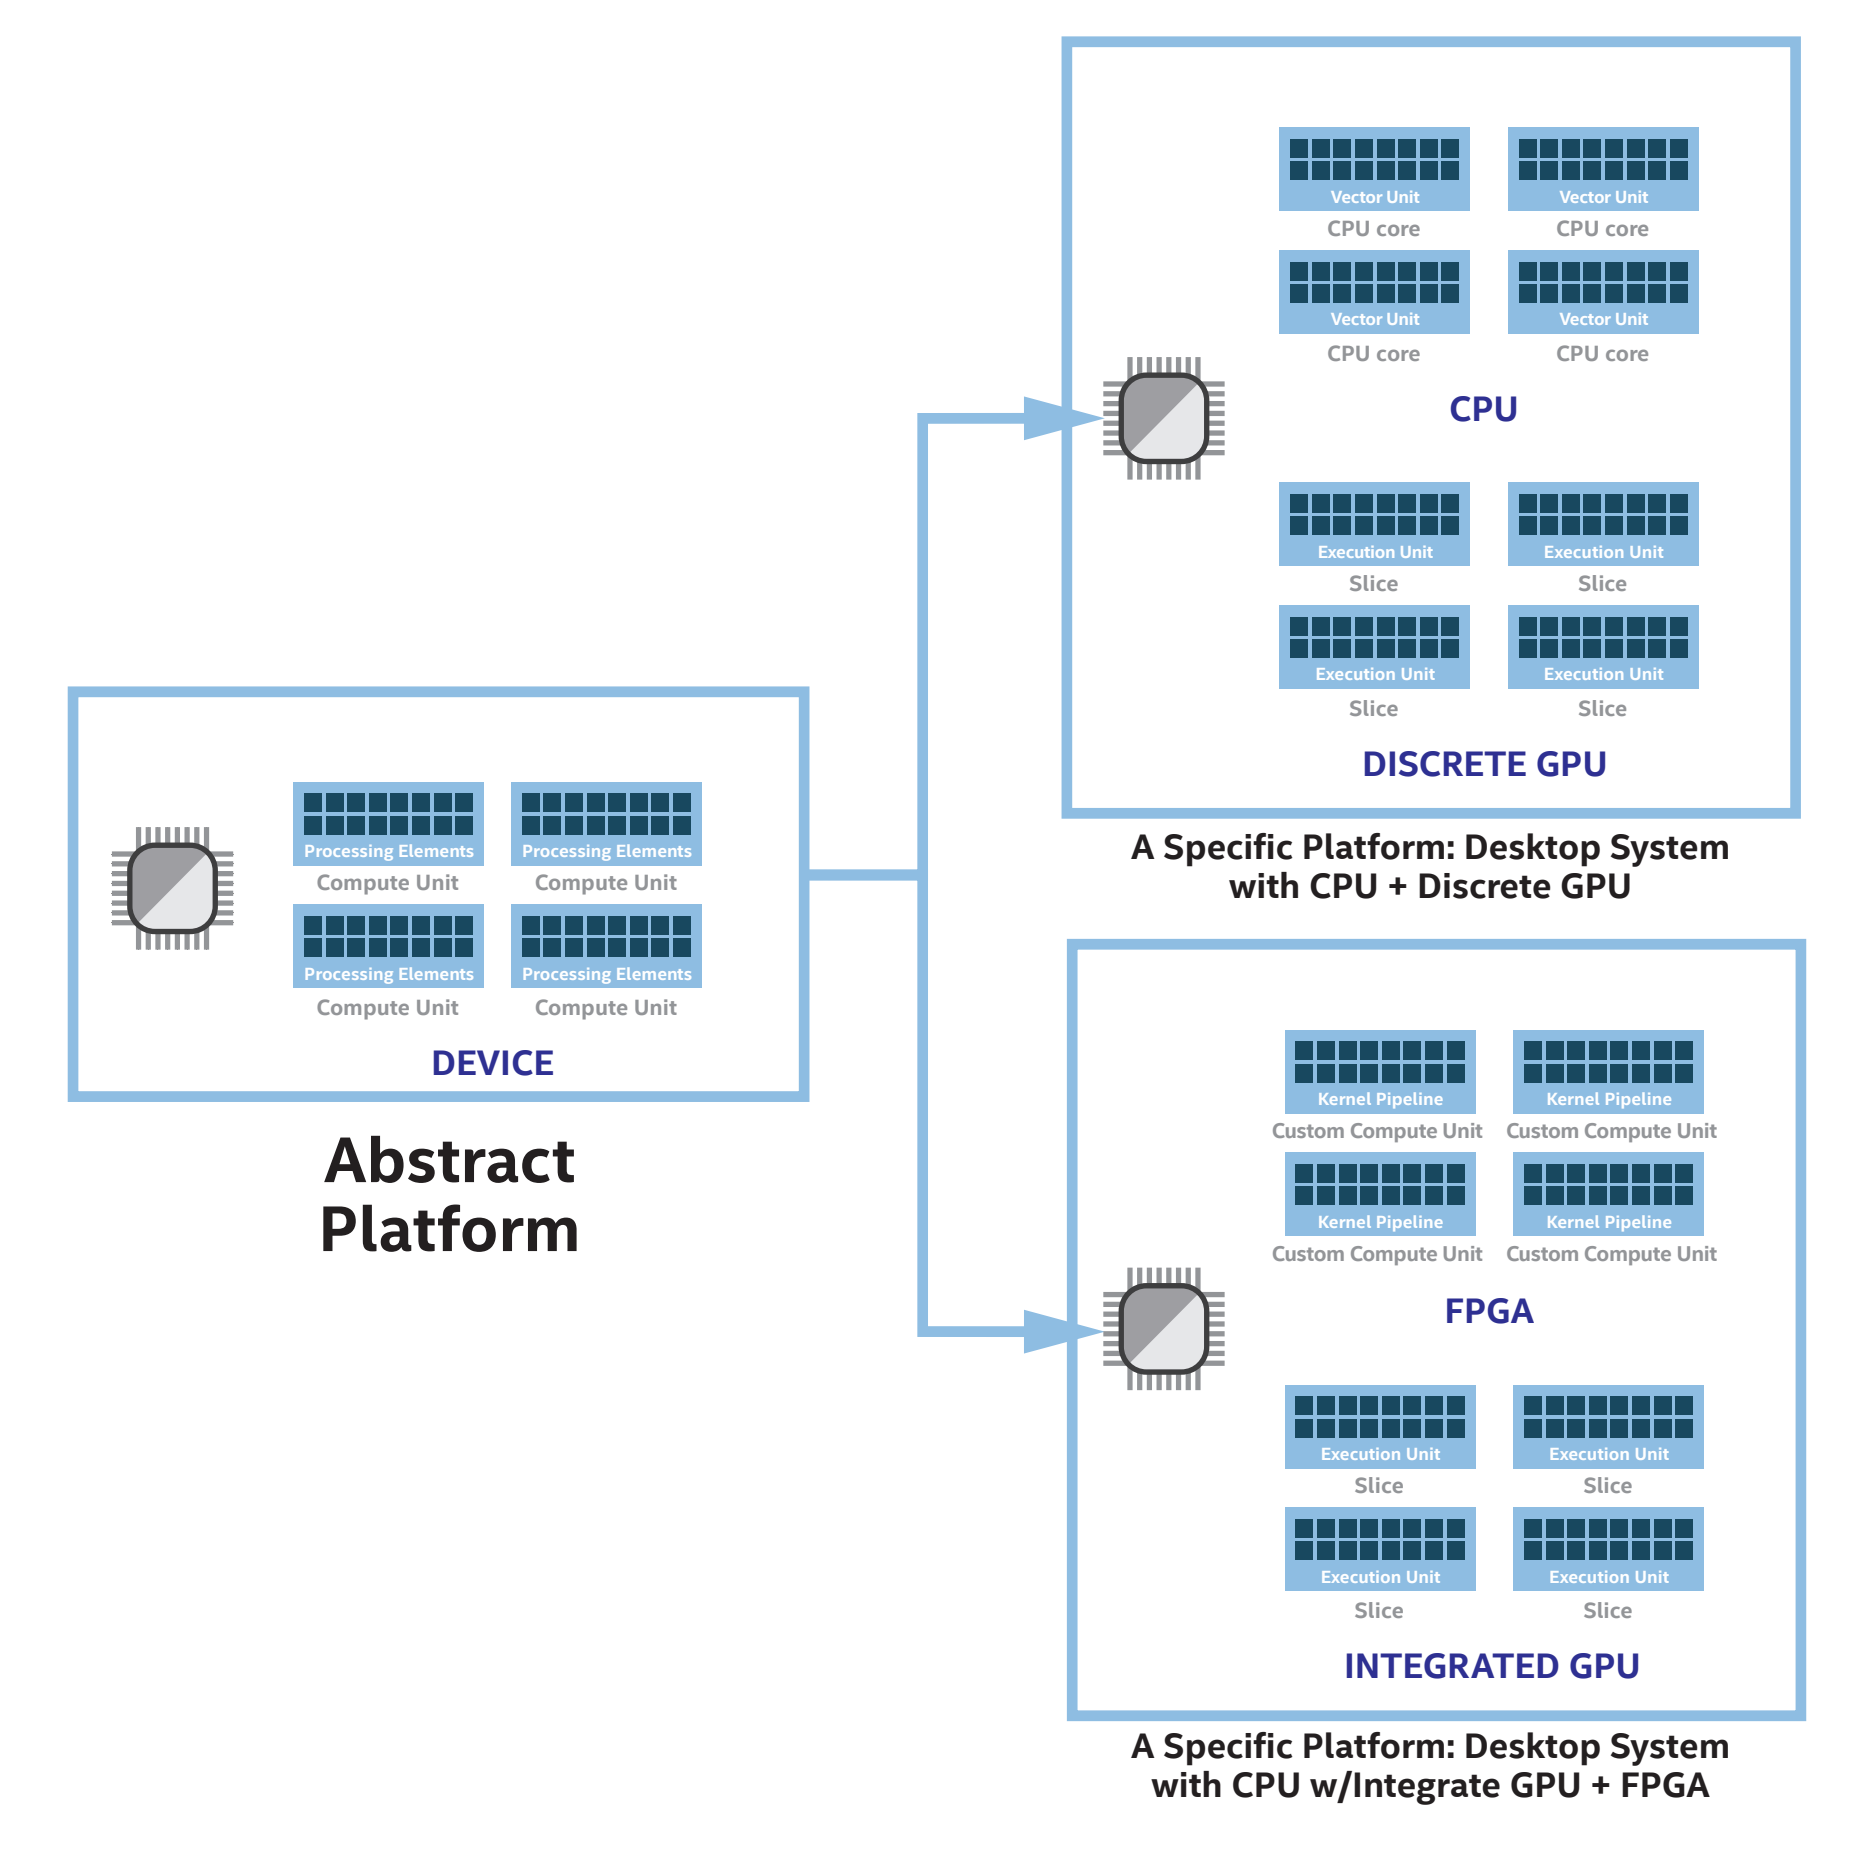
\includegraphics[width=1.\textwidth]{content/chapter-13/images/2}
\end{center}

\hspace*{\fill} \par %插入空行
\textbf{Multiarchitecture Binaries}

Since our goal is to have a single-source code to support a heterogeneous machine, it is only natural to want a single executable file to be the result.\par

A multiarchitecture binary (aka a fat binary) is a single binary file that has been expanded to include all the compiled and intermediate code needed for our heterogeneous machine. The concept of multiarchitecture binaries is not new. For example, some operating systems support multiarchitecture 32-bit and 64-bit libraries and executables. A multiarchitecture binary acts like any other a.out or A.exe we are used to—but it contains everything needed for a heterogeneous machine. This helps to automate the process of picking the right code to run for a particular device. As we discuss next, one possible form of the device code in a fat binary is an intermediate format that defers the final creation of device instructions until runtime.\par

\hspace*{\fill} \par %插入空行
\textbf{Compilation Model}

The single-source nature of SYCL and DPC++ allows compilations to act and feel like regular C++ compilations. There is no need for us to invoke additional passes for devices or deal with bundling device and host code. That is all handled automatically for us by the compiler. Of course, understanding the details of what is happening can be important for several reasons. This is useful knowledge if we want to target specific architectures more effectively, and it is important to understand if we need to debug a failure happening in the compilation process.\par

We will review the compilation model so that we are educated for when that knowledge is needed. Since the compilation model supports code that executes on both a host and potentially several devices simultaneously, the commands issued by the compiler, linker, and other supporting tools are more complicated than the C++ compilations we are used to (targeting only one architecture). Welcome to the heterogeneous world!\par

This heterogeneous complexity is intentionally hidden from us by the DPC++ compiler and “just works.”\par

The DPC++ compiler can generate target-specific executable code similar to traditional C++ compilers (ahead-of-time (AOT) compilation, sometimes referred to as offline kernel compilation), or it can generate an intermediate representation that can be just-in-time (JIT) compiled to a specific target at runtime.\par

The compiler can only compile ahead of time if the device target is known ahead of time (at the time when we compile our program). Deferring for just-in-time compilation gives more flexibility, but requires the compiler and the runtime to perform additional work while our application is running.\par

\begin{tcolorbox}[colback=red!5!white,colframe=red!75!black]
DPC++ compilation can be “ahead-of-time” or “just-in-time.”
\end{tcolorbox}

By default, when we compile our code for most devices, the output for device code is stored in an intermediate form. At runtime, the device handler on the system will just-in-time compile the intermediate form into code to run on the device(s) to match what is available on the system.\par

We can ask the compiler to compile ahead-of-time for specific devices or classes of devices. This has the advantage of saving runtime, but it has the disadvantage of added compile time and fatter binaries! Code that is compiled ahead-of-time is not as portable as just-in-time because it cannot adjust at runtime. We can include both in our binary to get the benefits of both.\par

Compiling for a specific device ahead-of-time also helps us to check at build time that our program should work on that device. With just-in-time compilation, it is possible that a program will fail to compile at runtime (which can be caught using the mechanisms in Chapter 5). There are a few debugging tips for this in the upcoming “Debugging” section of this chapter, and Chapter 5 details how these errors can be caught at runtime to avoid requiring that our applications abort.\par


Figure 13-2 illustrates the DPC++ compilation process from source code to fat binary (executable). Whatever combinations we choose are combined into a fat binary. The fat binary is employed by the runtime when the application executes (and it is the binary that we execute on the host!). At times, we may want to compile device code for a particular device in a separate compile. We would want the results of such a separate compilation to eventually be combined into our fat binary. This can be very useful for FPGA development when full compile (doing a full synthesis place-and-route) times can be very long and is in fact a requirement for FPGA development to avoid requiring the synthesis tools to be installed on a runtime system. Figure 13-3 shows the flow of the bundling/unbundling activity supported for such needs. We always have the option to compile everything at once, but during development, the option to break up compilation can be very useful.\par

Every SYCL and DPC++ compiler has a compilation model with the same goal, but the exact implementation details will vary. The diagrams shown here are for the DPC++ compiler toolchain.\par

One DPC++-specific component is shown in Figure 13-2 as the integration header generator that will not be mentioned again in this book. We can program without ever needing to know what it is or what it does. Nevertheless, to satisfy the curious, here is a little information: The integration header generator generates a header file providing information about SYCL kernels found in the translation unit. This includes how the names of SYCL kernel types map to symbolic names and information about kernel parameters and their locations within the corresponding lambda or functor object created by the compiler to capture them. The integration header is the mechanism used to implement the convenient style of kernel invocation from host code via C++ lambda/functor objects, which frees us from the time-consuming task of setting individual arguments, resolving kernels by name, and so on.\par

\hspace*{\fill} \par %插入空行
Figure 13-2. Compilation process: Ahead-of-time and just-in-time options
\begin{center}
	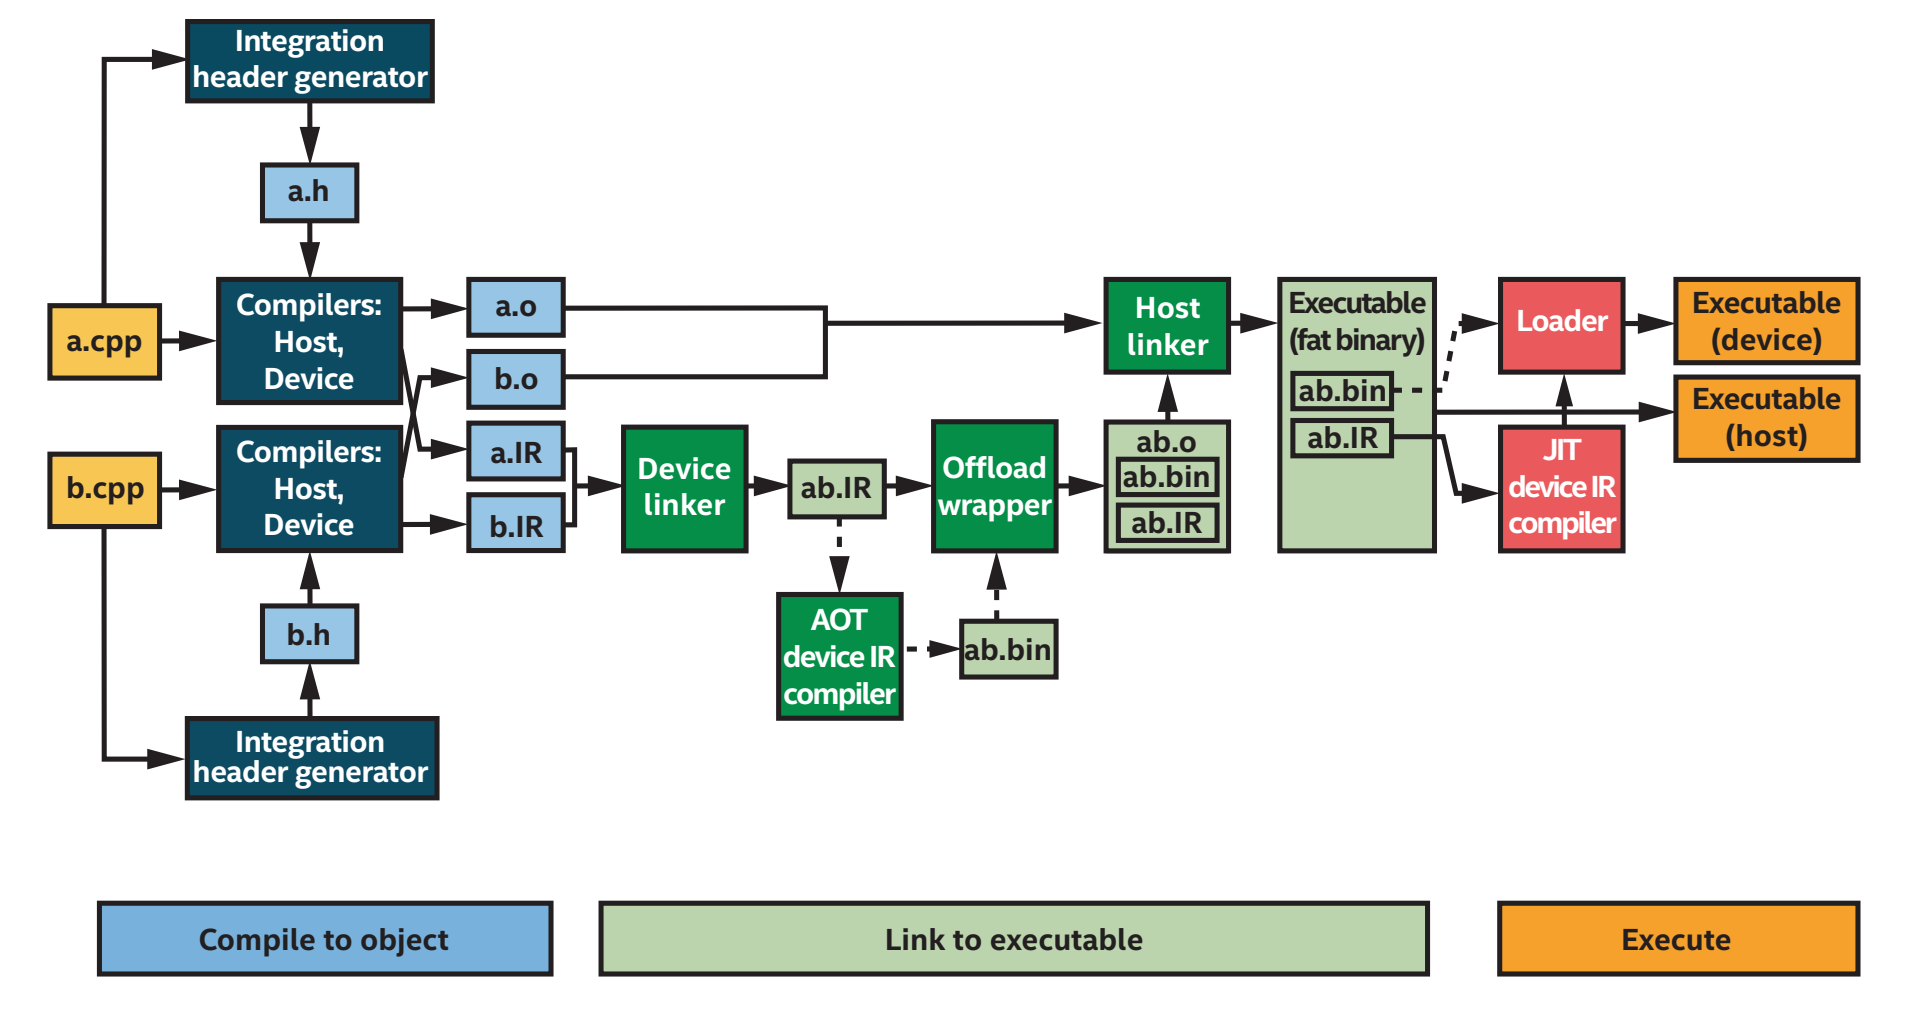
\includegraphics[width=1.\textwidth]{content/chapter-13/images/3}
\end{center}

\hspace*{\fill} \par %插入空行
Figure 13-3. Compilation process: Offload bundler/unbundler
\begin{center}
	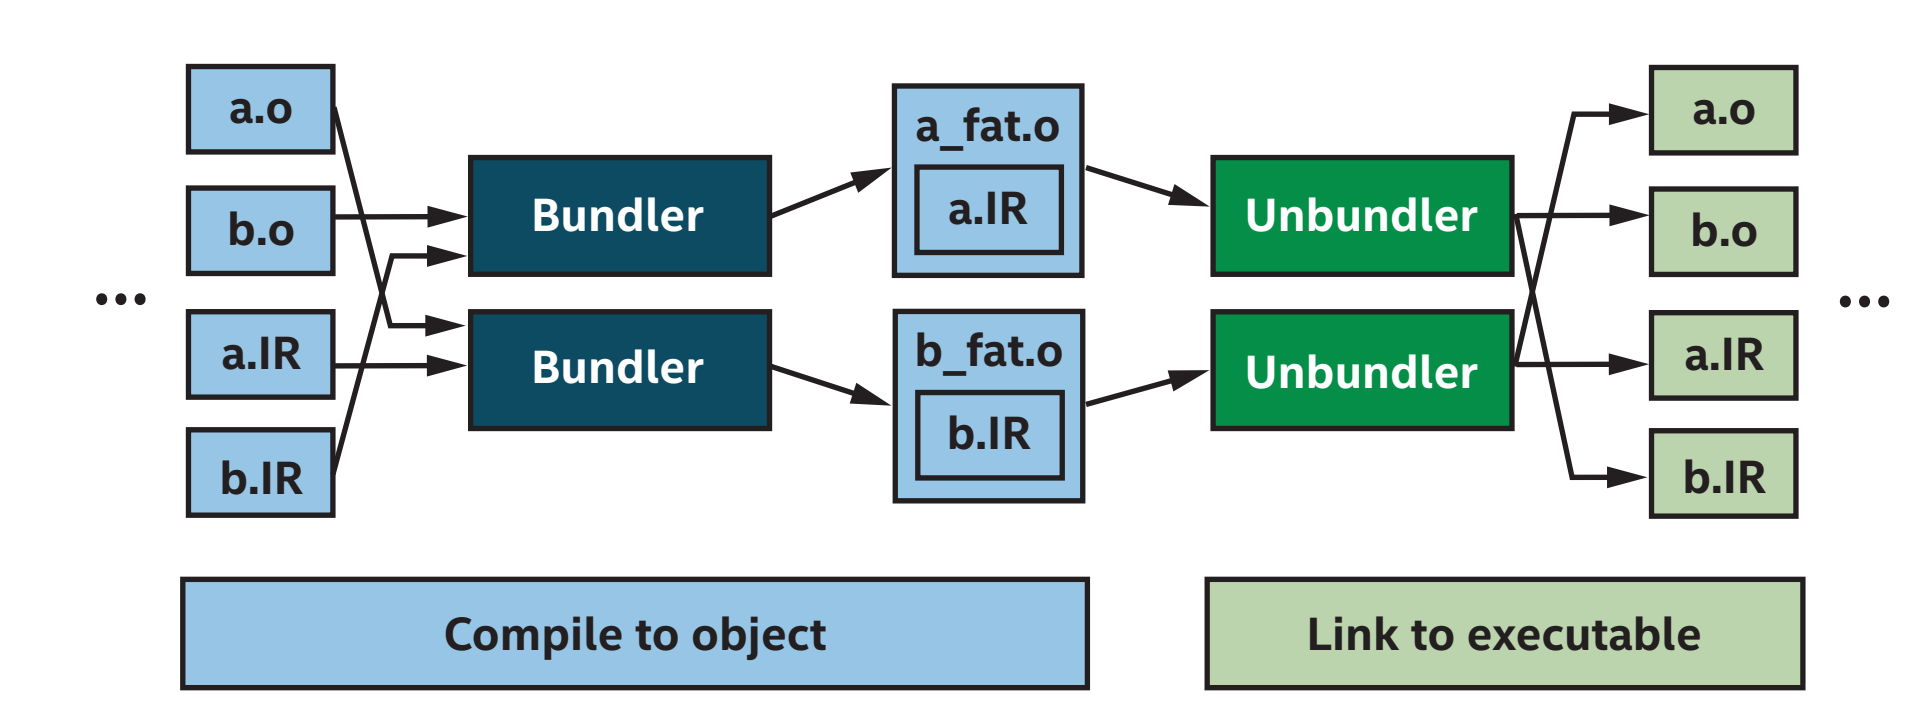
\includegraphics[width=1.\textwidth]{content/chapter-13/images/4}
\end{center}




































